\documentclass{bfh}

\title{Project 2}
\subtitle{Bitmessage -- Communication Without Metadata}
\author{Christian Basler}
\date{\today}

\begin{document}
  \maketitle

\begin{figure}[h]
\includegraphics[width=0.2\textwidth]{logo.png}
\centering
\end{figure}

  \tableofcontents

  \section{Synopsis}



  % Section basics
    \section{Introduction}

  \subsection{What is Metadata?}

  While encryption technology like PGP or S/MIME provides a secure way to protect content from prying eyes, ever since Edward Snowdens whistleblowing we learned that metadata --- most notably information about who communicates with whom --- is equally interesting and much easier to analyze.

  There are a few examples where meta data might be enough to get you in trouble. If you write to someoune in the IS, you might not be able to fly the next time you want to visit the U.S. The no-fly list doesn't care if you're a journalist, or had no clue that this person was a terrorist.

  If Samsung knows Apple talks excessively with the sole producer of this nifty little sensor, they don't need the details --- the S7 will sport one of those, too. (Failing to see that Apple used it to build a car.)

  \subsection{How Can We Hide Metadata?}

  With e-mail, we can only prevent this by encrypting the connection to the server as well as between servers. Therefore we can only hope that both our and the recipient's e-mail provider are both trustworthy as well as competent.\footnote{Of course they should be free as well.}

  With Bitmessage we send a message to a sufficiently large number of participants, with the intended recipient among them. Content is encrypted such as only the person in possesion of the private key can decrypt it. All participants try to do this in order to find their messages.

  The protocol is described in detail in my Seminar paper.


  \section{Goal}

  At the moment, there aren't many implementations apart from the official clients. Especially two things are missing: a multi purpose Java library and a usable mobile client. My goal for my \textit{Project 2} is to create the library, to be used next semester as a starting point for an Android\textsuperscript{\texttrademark} client in my Bachelor Thesis.


  \section{Issues}

  \subsection{Proof of Work}

  Proof of work is needed for a message to be distributed within the Bitmessage network. This is to protect both the network itself from denial of service attacks and the users from spam.


  \section{Architecture}

  \subsection{Ports and Adapters}

  The library uses a ports and adapters architecture, which allows us to easily replace some implementations that might be platform dependent, such as storage or proof of work calculation.

  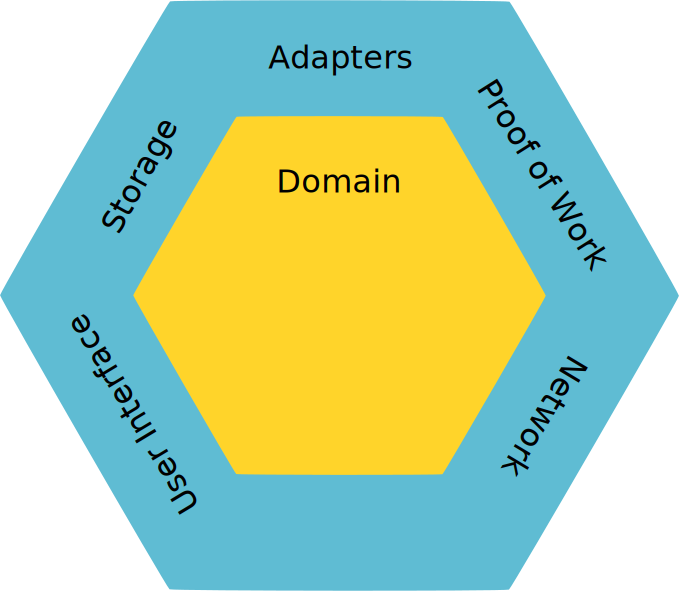
\includegraphics[width=\textwidth]{images/ports_and_adapters.pdf}

  The big advantage of this approach is that it's easy to test the core as well as each adapter by itself.


  \subsection{Network Management}


  \section{Discussion}


  \appendix
  \addcontentsline{toc}{section}{Appendix}
  \section*{Appendix}
  \renewcommand{\thesubsection}{\Alph{subsection}}


  \subsection{JavaDoc Documentation}


  \subsection{Literature}


\end{document}